\documentclass[12pt]{scrartcl}

\usepackage[
  a4paper, mag=1000,
  left=2cm, right=1cm, top=2cm, bottom=2cm, headsep=0.7cm, footskip=1.27cm
]{geometry}

\usepackage[T2A]{fontenc}
\usepackage[utf8]{inputenc}
\usepackage[english,russian]{babel}
\usepackage{cmap}
\usepackage{amsmath}
\usepackage{tabularx}
\usepackage{graphicx}
\usepackage{array}
\IfFileExists{pscyr.sty}{\usepackage{pscyr}}{}
\usepackage[parfill]{parskip}
\usepackage{lastpage}
\usepackage{setspace} % single spacing between lines
\usepackage{blindtext} % for generated text - can remove
\usepackage{titlesec} % set header spacing
\usepackage{listings} %listing
\usepackage{color}
\definecolor{commentGreen}{rgb}{0,0.6,0}

\setlength{\parindent}{15pt} % paragraph indent

\lstdefinestyle{cpp}{
  language=c++,
  basicstyle=\small\ttfamily,
  breakatwhitespace=true,
  breaklines=true,
  showstringspaces=false,
  keywordstyle=\color{blue}\ttfamily,
  stringstyle=\color{red}\ttfamily,
  commentstyle=\color{commentGreen}\ttfamily,
  morecomment=[l][\color{magenta}]{\#},
  xleftmargin=1cm
}

\titlespacing{\section}{0pt}{\parskip}{-\parskip}
\titlespacing{\subsection}{0pt}{\parskip}{-\parskip}
\titlespacing{\subsubsection}{0pt}{\parskip}{-\parskip}

\usepackage[numbered]{bookmark}
\clubpenalty=10000
\widowpenalty=10000

\usepackage{fancybox,fancyhdr}
\pagestyle{fancy}
\fancyhf{}
\fancyhead[C]{\small{Олимпиадное программирование (средний уровень). Тренировка 05\\ Летняя компьютерная школа ``КЭШ'', 6--26 августа 2016 года}}

%user-defined commands

\newcommand{\inputFile}{стандартный ввод}
\newcommand{\outputFile}{стандартный вывод}

\begin{document}

\singlespacing

\section*{Задача A. Смертельные шахматы }

\begin{tabularx}{\textwidth}{l l X}
    Имя входного файла: & \texttt{\inputFile} \\
    Имя выходного файла: & \texttt{\outputFile} \\
    Ограничение по времени: & $2$ секунды \\
    Ограничение по памяти: & $256$ мегабайт \\
\end{tabularx}

\begin{figure}[h]
	\centering
   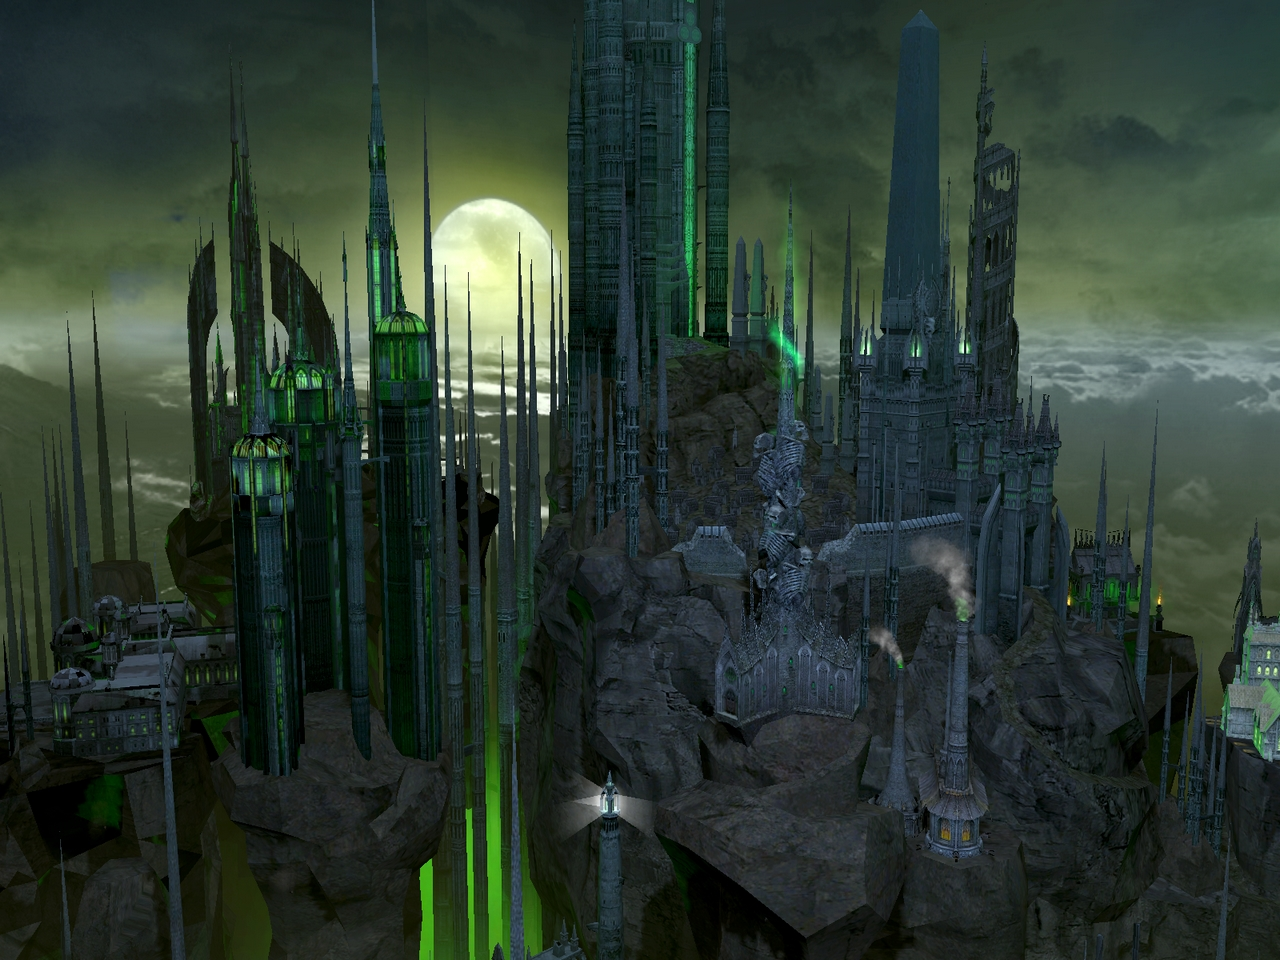
\includegraphics[width=0.6\linewidth]{deathCastle}
\end{figure}

Некромант Золтон хочет пополнить свою армию нежити, чтобы победить соседнее королевство эльфов. Для этого ему необходимо превратить солдатов других рас, которых он нанял, в скелетов или призраков при помощи ``Преобразователя нежити''. Но магия пребразователя не бесконечна, поэтому ему необходимо выбрать самых сильных, ловких и умных войнов. Для проверки ума некромант решил организовать турнир по костянным шахматам. Целью игры является уничтожение всех фигур соперника всего лишь одной  --- призрачной ящерицей. Ящерица может ходит только буквой ``Г''. Фермер Вилли боится не пройти испытание, так как совсем не умеет играть в шахматы. Помогите не очень умному, но инициативному крестьянину присоединиться к величайщей армии нежити. Для этого вам необходимо узнать всевозможные ходы из заданной точки и сообщить координаты новых точек Вилли. 

\subsection*{Формат входных данных}
Вводятся два числа $x$ и $y$~---~координаты начального положения призрачной ящерицы ($1 \leq x,y \leq 8$). 

\subsection*{Формат выходных данных}
Выведите координаты всех возможных клеток, в которых окажется ящерица после хода Вилли. Порядок вывода любой. 

\subsection*{Примеры}

\texttt
{
	\begin{tabularx}{0.9\textwidth}{| X | X |}
       \hline
       \multicolumn{1}{|c|}{\inputFile} & \multicolumn{1}{c|}{\outputFile} \\ 
       \hline 
       	1 4 &
       \parbox[t]{\textheight}
		{       
       	2 6   \\
	   	3 5	  \\
	   	2 2	  \\
	   	3 3	  \\
	   } \\
       \hline
    \end{tabularx}
}

\newpage

\section*{Задача B. Темные письмена}

\begin{tabularx}{\textwidth}{l l X}
    Имя входного файла: & \texttt{\inputFile} \\
    Имя выходного файла: & \texttt{\outputFile} \\
    Ограничение по времени: & $2$ секунды \\
    Ограничение по памяти: & $256$ мегабайт \\
\end{tabularx}

\begin{figure}[h]
	\centering
   
\includegraphics[width=0.4\linewidth]{Sinitar}
\end{figure}

В замке великого чернокнижника Синитара есть библиотека с обширной коллекцией редких магических свитков. При очередной инспекции библиотеки колдуны обнаружили древний манускрипт, который описывает ритуал, по их догадкам позволяющий вызвать самую первую колдунью Эрин. По легендам она обладала небывалой силой и могла в одиночку стереть целые королевства с лица земли. Так как темные эльфы уже давно находятся в затяжной войне с демонами, призыв столь могущественного союзника явно сыграл бы им на руку, но свиток настолько ветхий, что его почти невозможно прочитать. Лучшие волшебники королевства без отдыха и сна корпели над восстановлением содержимого манускрипта, но так и не смогли целиком его восстановить. Они сообщили о результатах своему повелителю. Синитар не признает поражений и потому, он приказал позвать лучшие умы всех известных ему миров. Одним из таких счастливчиков стали вы. Доработайте восстановленное содержание ритуала, для того, чтобы оно стало правильным и помогло вызвать могучую силу. Но будьте осторожны, хоть одна ошибка может привести к ужасным последствиям и уничтожить все на свете. 

\subsection*{Формат входных данных}
Вам дан текст манускрипта, восстановленный колдунами:

\lstset{style=cpp}

\begin{lstlisting}
include<iostream> include<cmath>
const int count = 10;
int main() { array[isempty???]: of integer;
for(int i=-230; i<=cout; +-+i+-+-){cin>>array[i]<<array[i];}cout<<array[i]<<' ';
int result; for(int i=0;i<=count;i++){result+=array[i]}
cout<<"Summ: "<<result<endl;
int max=INT32_MIN;    //INT32_MIN - min value of int
int min=INT32_MAX;    //INT32_MAX - max value of int
for(int i=0;i<=10;i++){if(array[i]>max)max = array if(i less min);min=array[i] fi}
cout<<"MIN: "<<max<<' '<<"MAX: "<<min<<ldne;loob prime!=true;
for(int i=0;i<;i++){int end=sqrt(array[i]);prime=true;for(int j=0;j<=end;j++) {
if(array[i]%j==0) {
break;
}
while(!prime)cout<<array[i]<<"is prime;"<<endl;}
cout<<endl;
}))))}}}}}
\end{lstlisting}


\subsection*{Формат выходных данных}
На выходе вы должны получить правильное описание ритуала, который вызовет ведьму. 
Известно, что ритуал состоит из нескольких шагов:
\begin{enumerate}
	\item нужно привести 10 гидр и посчитать для каждой количество голов
	\item посчитать сколкьо всего голов будет находится в ритуальном кругу
	\item узнать гидру, с наименьшим количеством голов и с наибольшим, чтобы поставить их друг напротив друга
	\item узнать, кто из них обладает характеристикой ``простота''
\end{enumerate}

\subsection*{Примечание}
Известно, что каждое задание выводится с новой строки и содержит пробелы между всеми словами и значениями.



\newpage
\section*{Задача C. Ярость}

\begin{tabularx}{\textwidth}{l l X}
    Имя входного файла: & \texttt{\inputFile} \\
    Имя выходного файла: & \texttt{\outputFile} \\
    Ограничение по времени: & $2$ секунды \\
    Ограничение по памяти: & $256$ мегабайт \\
\end{tabularx}

\begin{figure}[h]
	\centering
  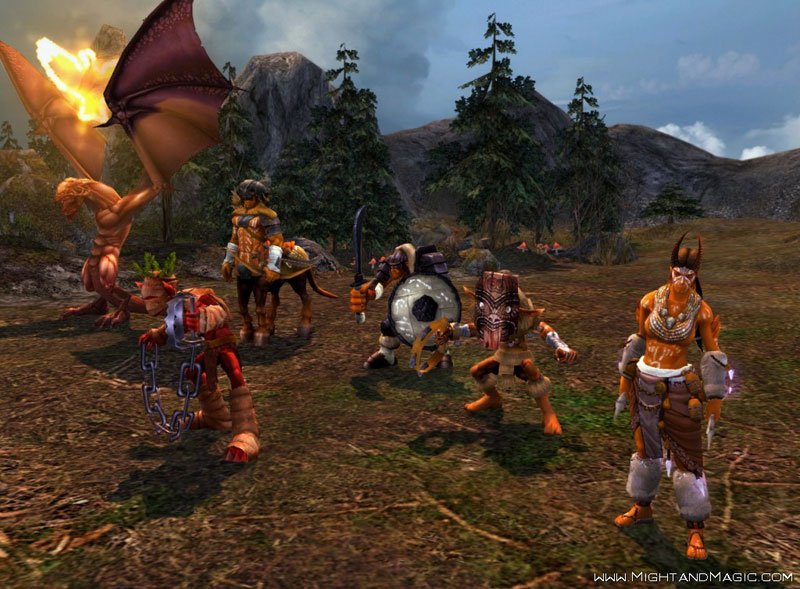
\includegraphics[width=0.6\linewidth]{orks}
 \end{figure}

У орков есть необычная особенность~---~ярость, она помогает им биться сильнее или слабее.Во время сражения они становятся яростнее, если наносят удар первыми и теряют ее, если на них напали. После сражения с мастерами лука Тилсек задался вопросом, а как у его войнов менялся уровень ярости с течением битвы. Он знает, сколько раз у любого его война изменялась ярость и на сколько преобразовывалось значение, но не имеет ни малейшего понятия, когда она убывала, а когда выростала. Тилсек так же имеет данные о текущем уровне ярости каждого солдата и знает, что в бой они шли совершенно спокойные и умиротворенные(то есть уровень ярости был на нуле). Помогите главе орков, который дружит с мечом больше, чем с арифметикой, разобраться, как изменялась яростность любого его война.

\subsection*{Формат входных данных}
В первой строке находятся числа $N(2 \leq N \leq 12$) и $S(-1 000 000 \leq S \leq 1 000 000)$, означающие количество изменений и текущая яростность, соотвественно. В следующей строке $N$ чисел через пробел~---~величину каждого изменения$(0 \leq X_i \leq 50 000)$.

\subsection*{Формат выходных данных}
Если получить требуемый результат невозможно, вывести "No solution". Если можно, то вывести равенство. Если решение не единственное, вывести любое. Числа и знаки нужно выводить через пробел.

\texttt
{
	\begin{tabularx}{0.9\textwidth}{| X | X |}
       \hline
       \multicolumn{1}{|c|}{\inputFile} & \multicolumn{1}{c|}{\outputFile} \\ 
       \hline 
        \parbox[t]{\textheight}
       	{
       	3 10 \\
		15 25 30 \\
		} &
		15 + 25 - 30 = 10 \\
		\hline
       \parbox[t]{\textheight}
		{       
       	2 100 \\
		10 10 \\
	   } & 
	   No solution \\
       \hline
    \end{tabularx}
}


\end{document}
